\documentclass[twocolumn,a4paper,10pt]{article}
\usepackage[print,sort]{standalone}
\usepackage[T1]{fontenc}
\usepackage[utf8]{inputenc}
\usepackage[english]{babel}
\usepackage{graphicx,float}
\usepackage{amssymb}
\usepackage{amsmath,cancel}
\usepackage{mathrsfs}
\usepackage{epstopdf}
%\usepackage{subcaption}
%\usepackage{slashed}
%\usepackage{hhline}
%\usepackage[margin=1.2in]{geometry}
\usepackage[hidelinks]{hyperref}
%\usepackage{wrapfig}


\hfuzz=5pt
%\usepackage[dvips]{graphicx}

% Variable enumeration
\usepackage{enumerate}

% Use all allowed space
\addtolength{\hoffset}{-0.5cm}
\addtolength{\textwidth}{1.0cm}
\addtolength{\voffset}{-1.5cm}
\addtolength{\textheight}{3cm}
\setlength{\columnsep}{0.5cm}

% Remove Abstract titile for abstract
%\renewcommand{\abstractname}{}

\author{Even S. Håland}

\title{How light can sleptons be?}

\begin{document}

% Abstract construction for using both columns in two-column format
\twocolumn[
\begin{@twocolumnfalse}
  \maketitle
  \begin{abstract}
Several searches for production of sleptons has been performed in collider experiments such as the currently running LHC, and its predecessor LEP. In this article we investigate the limits on the slepton mass(es) set by these experiments, with special emphasis on how light sleptons are allowed to be with the current limits. We also take a look at the models used in these searches, how these compare to the MSSM, and how the limits from these searches can be related to the sleptons in the MSSM.
 \end{abstract}
  \vspace{5mm}
\end{@twocolumnfalse}
]

\section{Introduction}

The Minimal Supersymmetric Standard Model (MSSM) is the smallest possible supersymmetric 
of the Standard Model (SM). Roughly explained the MSSM introduces one superpartner for each 
SM particle (with some complications in the Higgs sector), and the SM particles and their 
superpartners (often called sparticles) differ by $\frac{1}{2}$ in spin. 
The sparticles we will focus on here are the superpartners of the SM leptons, which are scalar (i.e. 
spin-$0$) particles called \textit{sleptons}, and we will focus mainly on the first two generations of 
charged sleptons, i.e. selectrons ($\tilde{e}$) and smuons ($\tilde{\mu}$).  

In particle collider experiments, such as the Large Electron-Positron Collider (LEP) and the currently 
running Large Hadron Collider (LHC), several searches for production of sleptons have been done, but 
so far without any sign of their existence. The consequence of such "negative" searches is usually 
that new limits are put on the masses of the relevant sparticles (or other parameters).              

In this article we will try to summarize the current status of the limits on the selectron and smuon 
masses. However, since the MSSM is a quite complicated model with $105$ free parameters, one has to make 
assumptions and simplifications when setting limits, and these are (of course!) somewhat different from 
analysis to analysis. We will therefore also take a look at which assumptions are made in the different  
analyses. But before all this, let us look at how sleptons are described in the MSSM.          

\section{Sleptons in the MSSM}

As mentioned in the introduction the sleptons are the scalar superpartners of the SM leptons. In the 
SM there is an important difference between left- and right-handed chiral states, in that the 
left-handed leptons are organized in weak isospin doublets, while the right-handed ones are singlets 
(i.e. they do not transform under $SU(2)_L$). This mean that, when constructing a supersymmetric theory, 
we need to introduce separate superpartners for the left- and right-handed leptons. For this reason we 
talk about left- and right-handed sleptons ($\tilde{\ell}_L$ and $\tilde{\ell}_R$) even though they are 
scalar particles. 

This has some consequences when we are breaking SUSY. As we know, SUSY must be a broken symmetry, 
since otherwise particles and sparticles would have equal masses, meaning that SUSY would have been 
discovered a long time ago. For the first two generations of (charged) sleptons (neglecting the 
Yukawa coupling) the mass is given as
\begin{align}
m_{\tilde{\ell}}^2 = m_{\ell}^2 + (T_3 - Q\sin^2\theta_W)\cos 2\beta m_Z^2, 
\end{align}  
where $m_{\ell}$ is the  mass of the corresponding SM lepton, $T_3$ is weak isospin, $Q$ is 
electric charge, $\theta_W$ is the Weinberg angle, $\beta$ is given by the ration between the 
vacuum expectation values of the two Higgs doublets of the MSSM, and $m_Z$ is the mass of the $Z$-boson.
Interesting to notice is that $m_{\tilde{\ell}}$ depends on weak isospin, which is different for 
$\tilde{\ell}_L$ ($T_3 = -1/2$) and $\tilde{\ell}_R$ ($T_3 = 0$), meaning that their masses are 
different. The mass difference is given by 
\begin{align}
m_{\tilde{\ell}_L}^2 - m_{\tilde{\ell}_R}^2 = -\frac{1}{2}\cos 2\beta m_Z^2.  
\end{align}  
By convention we have $0 < \beta < \frac{\pi}{2}$, and it is (apparently, check this!) in the MSSM a 
common assumption that $\tan\beta > 1$, meaning that $\cos 2\beta < 0$, so 
\begin{align*}
m_{\tilde{\ell}_L}^2 > m_{\tilde{\ell}_R}^2. 
\end{align*} 
This mass splitting is however usually assumed to be small, and in experiments $\tilde{\ell}_R$ and 
$\tilde{\ell}_L$ are often (but not always) assumed to be mass degenerate. 

\section{Constrained models}

As mentioned in the introduction the MSSM has $105$ free parameters (plus the $19$ free parameters 
of the SM), which makes it somewhat difficult to use for phenomenological predictions and interpretation 
of experimental data. For this reason we need to consider constrained models, where the number of 
free parameters is drastically reduced. We will not go into much details here, but simply mention a 
few of the most popular once, which are also the most relevant for the analyses discussed later.  
This review is mainly based on ref. \cite{Simplified models}. 

The first model we should mention is a very popular one known as minimal supergravity (mSUGRA) or 
constrained MSSM (CMSSM). This model provides a mechanism for explaining SUSY breaking through 
gravitational interactions at Planck scale, and at GUT scale the model only depends on five free 
parameters,  
\begin{align*}
m_{1/2},\:\: m_0, \:\: A_0, \:\: \tan\beta \:\:\text{and}\:\: \text{sgn}(\mu), 
\end{align*}
where $m_{1/2}$ is a common gaugino mass, $m_0$ is a common scalar mass, $A_0$ is a universal tri-linear 
Yukawa coupling, $\tan\beta$ is the ratio between the vacuum expectation values for the two Higgs 
doublets of the MSSM and sgn$(\mu)$ is the sign of the Higgs mass parameter. The MSSM parameters at 
electroweak scale are obtained by the renormalization group equation.      

Another model we should mention is the phenomenological MSSM (pMSSM), which is a way of limiting the 
MSSM parameter space by including three assumptions; \textit{i)} No new sources of CP-violation, 
\textit{ii)} no flavour changing neutral currents, \textit{iii)} first and second generation universality. 
The last assumption implies that the masses of first and second generation sfermions are equal. With 
these assumptions the number of free parameters is reduced to $19$.  

Finally we should mention that for instance in recent searches by ATLAS (e.g. ref. \cite{ATLAS:2017}) 
so-called simplified models are used when interpreting the results. 

\section{Slepton production in particle colliders}

The MSSM is usually defined as conserving R-parity, given as  
\begin{align*}
R = (-1)^{2s + 3B + L}, 
\end{align*}
where $s$ is spin, $B$ is baryon number and $L$ is lepton number. This has the 
interesting consequences that sparticles will always be produced in pairs in particle colliders, 
the lightest sparticle (LSP) will be stable, and all other sparticles will (possibly via multiple steps) 
decay to the LSP. Conservation of R-parity (and some other quantum numbers) means that slepton searches 
target production of $\tilde{\ell}^+\tilde{\ell}^-$, and it is a very common assumption that the LSP is 
the lightest neutralino, $\tilde{\chi}_1^0$, which is an excellent candidate particle for dark matter. 
Often sleptons are assumed to decay directly to $\tilde{\chi}_1^0$, plus the corresponding SM lepton. 
The mass difference, 
\begin{align}
\Delta m = m_{\tilde{\ell}} - m_{\tilde{\chi}^0_1}, 
\label{eq:delta m}
\end{align}  
is in this case quite important, since it basically determines the momentum of the lepton, which is 
what you observe in the detector. Scenarios with small $\Delta m$ is in some experiments hard to study. 

In hadron colliders, such as the LHC, the cross section for slepton production is expected to be 
quite small, since the production of coloured (s)particles should be dominant, since hadrons (protons) 
are strongly interacting particles. 
However, if coloured sparticles are sufficiently heavy, production of sleptons (and other electroweak 
sparticles) could be the leading SUSY production channel. At leading order a pair of sleptons can be 
produced through $q\bar{q}$ annihilation to a virtual $Z/\gamma$, which splits into 
$\tilde{\ell}^+\tilde{\ell}^-$ ($s$-channel). In lepton colliders there is a similar $s$-channel, only 
with $e^+e^-$ annihilation, but in addition there is also a $t$-channel with neutralino exchange 
available at leading order.  

\section{Slepton mass limits}

Now that we have introduced some theory and phenomenology concerning sleptons it is time to move into 
the more experimental details. We will mainly focus on searches done at LEP and the LHC, as the best 
current limits stems from these experiments. We will take a look at what the actual limits are, and 
which assumptions that are made in the various searches.    

\subsection{LEP}

The Large Electron-Positron collider (LEP) was a $27$ km $e^+e^-$ collider at CERN running between 
$1989$ and $2000$, and is still the most powerful lepton collider ever built, with a peak energy of 
$209$ GeV. Although this is much less than the energy at which the LHC collides protons, and the 
total delivered luminosity is much smaller than in the LHC, it is interesting to notice that the 
LEP experiments still has the most general limits on the masses of both selectrons and smuons.  

An absolute lower limit on the selectron masses, $m_{\tilde{e}_L}$ and $m_{\tilde{e}_R}$,  within the 
MSSM is set by the ALEPH experiment in ref. \cite{ALEPH:2002} to be  
\begin{align*}
m_{\tilde{e}_R} & > 73 \:\: \text{GeV}, \\
m_{\tilde{e}_L} & > 107 \:\: \text{GeV},   
\end{align*}       
assuming R-parity conservation, and that $\tilde{\chi}_1^0$ is the LSP. It is also assumed that 
scalar masses and gaugino masses are unified to $m_0$ and $m_{1/2}$ respectively at GUT scale, and 
that $\tan\beta > 1$, as mentioned previously. Finally, mixing between $\tilde{e}_L$ and $\tilde{e}_R$ 
is neglected. It is however noteworthy that these limits are for \textit{any} $\Delta m$ (see eq. 
\ref{eq:delta m}). 

A limit on the smuon mass, $m_{\tilde{\mu}}$, was also set at LEP by the DELPHI experiment 
\cite{DELPHI:2003}. In this analysis it was assumed that only right-handed smuons would be light enough 
to be produced in LEP, so the limit only applies to $\tilde{\mu}_R$'s, and is given as 
\begin{align*}
m_{\tilde{\mu}_R} > 94 \:\: \text{GeV}, 
\end{align*}
interpreted in the CMSSM, for $1<\tan\beta <40$, $-1000\:\text{GeV} \leq \mu \leq 1000 \: \text{GeV}$, 
and assuming no mass splitting in the third generation of sfermions. (The last assumption is done because 
this gives the most conservative limit.) The limit applies to scenarios with  
$\Delta m > 10$ GeV.  Notice that, although the limit is for to right-handed smuons, since 
$m_{\tilde{\mu}_L}>m_{\tilde{\mu}_R}$, it also serves as a conservative limit on $m_{\tilde{\mu}_L}$. 
The same analysis (ref. \cite{DELPHI:2003}) also presents a mass limit on $\tilde{e}_R$ at $94$ GeV, 
which is higher than the one discussed previously by ALEPH. However, the DELPHI-analysis requires 
$\Delta m > 10$ GeV, so the ALEPH limit is still the most general one on $m_{\tilde{e}_R}$.   

\subsection{LHC}

The Large Hadron Collider (LHC) at CERN is the most powerful particle collider ever built. It  
spends most of its operational time accelerating and colliding protons, first in Run I ($2010$-$2012$) 
at $7$-$8$ TeV, and now in Run II (since $2015$) at $13$ TeV. With such a powerful accelerator a lot 
of people expected that the discovery of SUSY was just around the corner, but despite great efforts 
and plenty of searches no significant deviations from the Standard Model has been seen.

Searches for slepton production has been done by both ATLAS and CMS, which are the two multi-purpose 
experiments at the LHC. We will however stick to discussing results from the ATLAS experiment, because 
only ATLAS has set limits on the slepton mass using $13$ TeV data, while the limits from $8$ TeV analyses 
are quite similar for the two experiments. 

Two ATLAS analyses searching for slepton production is found in refs. \cite{ATLAS:2014} ($8$ TeV) and 
\cite{ATLAS:2017} ($13$ TeV). The limits in the latter are (much) stronger, but somewhat different 
models are used in the searches, which is why we should mention both of them.

In the $8$ TeV analysis results are interpreted in a pMSSM framework. It is (as usual) assumed that 
the lightest neutralino is the LSP, and also that the slepton is the next-to-lightest sparticle (NLSP) 
(i.e. it always decays as $\tilde{\ell}\rightarrow \tilde{\chi}_1^0 \ell$). The resulting exclusion 
limits for mass degenerate left- and right-handed sleptons is shown in Figure \ref{fig:ATLAS 8TeV}, 
with $m_{\tilde{\ell}}$ on the $x$-axis and $m_{\tilde{\chi}_1^0}$ on the $y$-axis.  
(Ref. \cite{ATLAS:2014} also contains separate limits for $\tilde{\ell}_L$ and $\tilde{\ell}_R$.)   
The red line marks the area excluded in this search, while the orange area is the limit from 
LEP on the $\tilde{\mu}_R$ mass. We see that excluded are has been quite significantly extended, but 
(as mentioned) the ATLAS search do not reach the smaller $\Delta m$'s.

\begin{figure}
\begin{center}
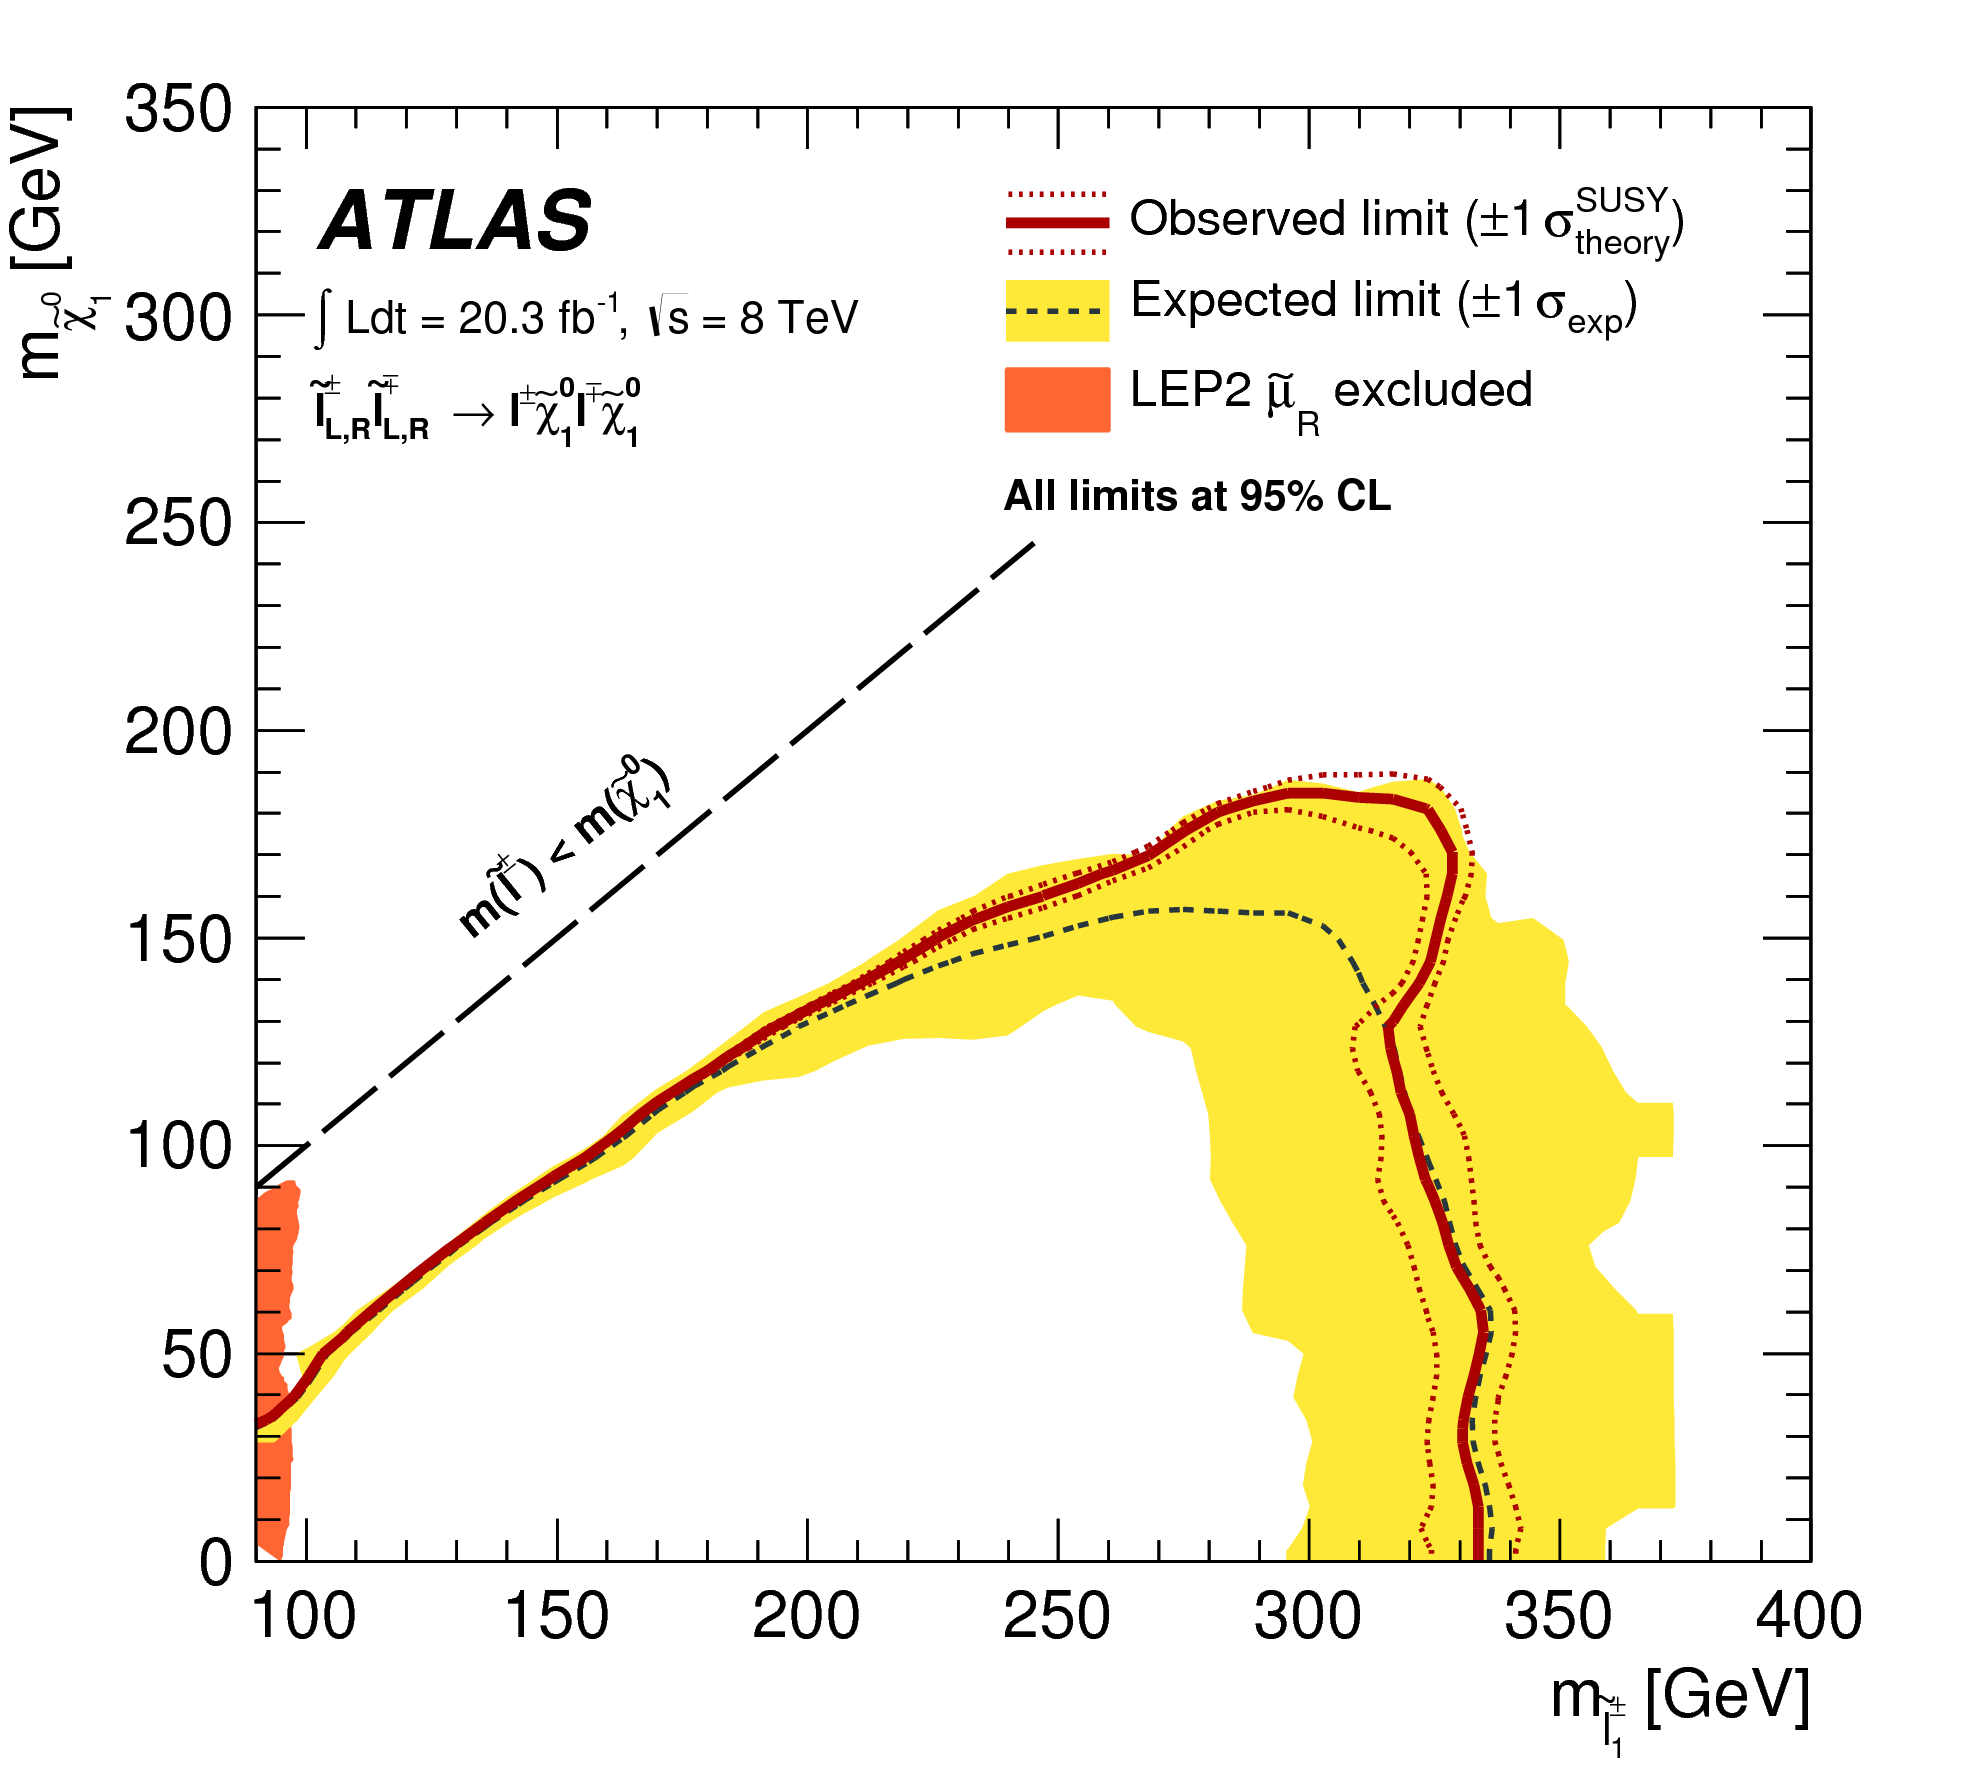
\includegraphics[scale=0.1]{Run1exclusion.png}
\caption{Exclusion limits on mass degenerate left- and right-handed sleptons from ATLAS at 
$8$ TeV \cite{ATLAS:2014}.}
\label{fig:ATLAS 8TeV}
\end{center}
\end{figure}  

Much of the same can also be said about the limits at $13$ TeV, shown in Figure \ref{fig:ATLAS 13TeV}, 
which were presented at the LHCP conference in May 2017. The green area is the previous limit at $8$ 
TeV, while the red on is the new observed limit. For this search a so-called simplified model is used, 
where the only free parameters are $m_{\tilde{\ell}}$ and $m_{\tilde{\chi}_1^0}$. It is noteworthy 
that, although the limits are extended by quite a bit, the limits in the compressed region (meaning 
small $\Delta m$) aren't improved at all compared to the $8$ TeV search.        

\begin{figure}
\begin{center}
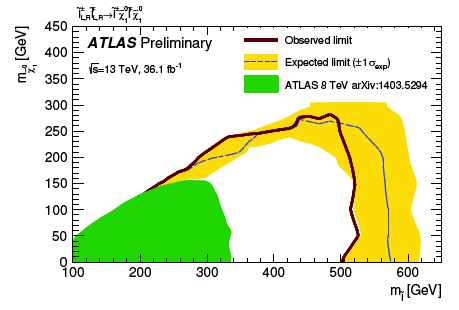
\includegraphics[scale=0.5]{Run2exclusion_new.png}
\caption{Exclusion limits on mass degenerate left- and right-handed sleptons from ATLAS at $13$ TeV 
\cite{ATLAS:2017}.}
\label{fig:ATLAS 13TeV}
\end{center}
\end{figure}

One might wonder why LEP, after all these years, still has better limits than the LHC experiments in the 
compressed region, and there is a very specific reason for this. ATLAS (and CMS) are primarily designed 
to search for new (heavy) particles. Such particles should, when decaying, lead to final state particles 
with high transverse momentum ($p_T$). The ATLAS detector is therefore designed to only keep events where 
such particles are present, and the trigger system \cite{ATLAS triggers} in ATLAS is really efficient 
only for leptons with $p_T \gtrsim 20$ GeV. Scenarios with low $\Delta m$ will typically lead to final 
states with so-called \textit{soft} leptons (i.e. low $p_T$), which are hard to study with ATLAS, hence 
sensitivities to such scenarios are low. 

However, a study done in ref. \cite{Compressed sleptons} shows that the LHC at $14$ TeV with $100$ 
fb$^{-1}$ of data could be sensitive to $\Delta m$'s as low as $3$ GeV up to 
$m_{\tilde{\ell}_L} \approx 150$ GeV. This study does however not make use of the traditional 
technique of studying final states with $\ell^+ \ell^-$ and MET, but makes use of events with 
energetic jets from initial state radiation (ISR). The idea is that the produced sleptons will recoil 
against these jets, leading to leptons with high $p_T$ also in low $\Delta m$ scenarios.        

\section{Summary and conclusions}

\begin{thebibliography}{9}

% Please take references when possible from SPIRES
% http://inspirehep.net/

\bibitem{Simplified models} 
  A. Djouadi et al. (1999). \\
  \href{https://arxiv.org/abs/hep-ph/9901246}{https://arxiv.org/abs/hep-ph/9901246}

\bibitem{ALEPH:2002}
  A. Heister et al. (2002), Phys.Lett. B544, 73-88. 
  \href{https://inspirehep.net/record/591226}{https://inspirehep.net/record/591226}
 
\bibitem{DELPHI:2003} 
  J. Abdallah et al. (2003), Eur.Phys.J.C31, 421-479. 
  \href{http://inspirehep.net/record/632738}{http://inspirehep.net/record/632738}	

\bibitem{ATLAS:2014} 
  G. Aad et al. (2014), JHEP 1405 071. \\
  \href{https://inspirehep.net/record/1286761}{https://inspirehep.net/record/1286761}

\bibitem{ATLAS:2017} 
  ATLAS Collaboration (2017), CONF-SUSY-2017-039. 
  \href{http://cds.cern.ch/record/2267406}{http://cds.cern.ch/record/2267406}      

\bibitem{ATLAS triggers}
  ATLAS Collaboration (2016). \\
  \href{https://arxiv.org/abs/1611.09661}{https://arxiv.org/abs/1611.09661}   

\bibitem{Compressed sleptons}
  A. Barr, J. Scoville (2015). \\ 
  \href{https://arxiv.org/abs/1501.02511}{https://arxiv.org/abs/1501.02511}
 
\end{thebibliography}

\end{document}
